\documentclass[../thesis.tex]{subfiles}
\begin{document}
	\section{Test Methodology}
	The experiment evaluates the results of the server by performing benchmark tests. In all the tests, we follow the one-factor-at-a-time experimental design \cite{oaat} to ensure the accuracy and effectiveness of tests.
	
	\subsection{Performance Testing}
	Performance Testing is a type of testing to ensure software applications will perform well under their expected workload. Features and Functionality supported by a software system is not the only concern. A software application's performance like its response time, reliability, resource usage and scalability do matter. The goal of Performance Testing is not to find bugs but to eliminate performance bottlenecks.
	\newline

	The focus of Performance Testing is checking a software program's:
 
	\begin{itemize}
		\item Speed - Determines whether the application responds quickly

		\item Scalability - Determines maximum user load the software application can handle.

		\item Stability - Determines if the application is stable under varying loads
	\end{itemize}

	Performance testing is popularly called as "Perf Testing" and is a subset of performance engineering. Performance testing is done to provide stakeholders with information about their application regarding speed, stability and scalability. More importantly, performance testing uncovers what needs to be improved before the product goes to market. Without performance testing, software is likely to suffer from issues such as: running slow while several users use it simultaneously, inconsistencies across different operating systems and poor usability. Performance testing will determine whether or not their software meets speed, scalability and stability requirements under expected workloads. Applications sent to market with poor performance metrics due to non existent or poor performance testing are likely to gain a bad reputation and fail to meet expected sales goals. Also, mission critical applications like space launch programs or life saving medical equipments should be performance tested to ensure that they run for a long period of time without deviations.
	\subsection*{Common Performance Problems}
	Most performance problems revolve around speed, response time, load time and poor scalability. Speed is often one of the most important attributes of an application. A slow running application will lose potential users. Performance testing is done to make sure an app runs fast enough to keep a user's attention and interest. Take a look at the following list of common performance problems and notice how speed is a common factor in many of them:
	\newline
    
	\begin{itemize}
		\item Long load time - Load time is normally the initial time it takes an application to start. This should generally be kept to a minimum. While some applications are impossible to make load in under a minute, Load time should be kept under a few seconds if possible.
		\newline
    
		\item Poor response time - Response time is the time it takes from when a user inputs data into the application until the application outputs a response to that input. Generally this should be very quick. Again if a user has to wait too long, they lose interest.
		\newline
    
		\item Poor scalability - A software product suffers from poor scalability when it cannot handle the expected number of users or when it does not accommodate a wide enough range of users. Load Testing should be done to be certain the application can handle the anticipated number of users.
		\newline
    
		\item Bottlenecking - Bottlenecks are obstructions in system which degrade overall system performance. Bottlenecking is when either coding errors or hardware issues cause a decrease of throughput under certain loads. Bottlenecking is often caused by one faulty section of code. The key to fixing a bottlenecking issue is to find the section of code that is causing the slow down and try to fix it there. Bottle necking is generally fixed by either fixing poor running processes or adding additional Hardware. Some common performance bottlenecks are CPU utilization
		Memory utilization, Network utilization, Operating System limitations, Disk usage.
	\end{itemize}
	\subsection*{Performance Testing Process}
	The methodology adopted for performance testing can vary widely but the objective for performance tests remain the same. It can help demonstrate that your software system meets certain pre-defined performance criteria. Or it can help compare performance of two software systems. It can also help identify parts of your software system which degrade its performance.
	\newline
    
	Below is a generic performance testing process -

	\begin{itemize}
		\item \textbf{Identify your testing environment} - Know your physical test environment, production environment and what testing tools are available. Understand details of the hardware, software and network configurations used during testing before you begin the testing process. It will help testers create more efficient tests.  It will also help identify possible challenges that testers may encounter during the performance testing procedures.

		\item \textbf{Identify the performance acceptance criteria} - This includes goals and constraints for throughput, response times and resource allocation.  It is also necessary to identify project success criteria outside of these goals and constraints. Testers should be empowered to set performance criteria and goals because often the project specifications will not include a wide enough variety of performance benchmarks. Sometimes there may be none at all. When possible finding a similar application to compare to is a good way to set performance goals.

		\item \textbf{Plan and design performance tests} - Determine how usage is likely to vary amongst end users and identify key scenarios to test for all possible use cases. It is necessary to simulate a variety of end users, plan performance test data and outline what metrics will be gathered.

		\item \textbf{Configuring the test environment} - Prepare the testing environment before execution. Also, arrange tools and other resources.

		\item \textbf{Implement test design} - Create the performance tests according to your test design.

		\item \textbf{Run the tests} - Execute and monitor the tests.

		\item \textbf{Analyze, tune and retest} - Consolidate, analyze and share test results. Then fine tune and test again to see if there is an improvement or decrease in performance. Since improvements generally grow smaller with each retest, stop when bottlenecking is caused by the CPU. Then you may have the consider option of increasing CPU power.
	\end{itemize}
	
	\subsection{Benchmark Test Methodology}
	Benchmark Testing is a type of testing done to give repeatable set of quantifiable result from which present and future software releases for specific functionality can be baselined or compared. It is a process used to compare the performance of software or hardware system also known as SUT (System Under Test). An SUT can be a Web-based application.
	\paragraph{}
	A benchmark must be repeatable. For instance, with every iteration of load test, if the response times varies too much, system performance be benchmarked. Response time needs to be stable amongst different load conditions.
	\paragraph{}
	A benchmark must be quantifiable. For example, user experience cannot be quantified in numbers, but time a user spends on a webpage due to good UI can be quantified.
	
	\subsection*{Importance of benchmark testing}
	At business level, benchmark testing can be helpful in determining

	\begin{itemize}
		\item How well a web-based application is performing with respect to the competitors
		\item It ensures that websites complies with standards and best practices
		\item It enables to evaluate third- party service providers prior to making a contracting decision
		\item Allows to figure out the mistakes to be avoided
		\item How different types of customers experience the response time and availability of a site.
	\end{itemize}
	\subsection{Phases of benchmark testing}
	\subsection*{Planning Phase}
	\begin{itemize}
		\item Identifying and prioritize standards and requirements
		\item Decide benchmark criteria
		\item Define benchmark test process
	\end{itemize}
	\subsection*{Analysis Phase}
	\begin{itemize}
		\item Identify root cause of error to improve quality
		\item Setting goals for test process
	\end{itemize}
	\subsection*{Integration Phase}
	\begin{itemize}
		\item Share outcomes with concerned person and get approval
		\item Establish functional goals
		\item Define benchmark test process
	\end{itemize}
	\subsection*{Action Phase}
	\begin{itemize}
		\item Develop test plan and documentation
		\item Implement actions specified in previous phases and monitor progress
		\item Run the process continuously
	\end{itemize}
	
	\subsection{Test setup}
	The benchmark test will be performed in three separate scenarios - CPU intensive task on local server, CPU intensive task on remote server and a SELECT database query on local server with a local database setup.
	
	The remote servers are hosted on DigitalOcean web server platform, with each technology having it's own dedicated server.
	
	\subsection{Testing the web technologies}
	According to one-factor-at-a-time experimental design, we make three fundamental tests - Calculate Value of Fibonacci and Fetch data from local DB and Fetch data from remote DB. Calculate Value of Fibonacci module calculates some value of Fibonacci and evaluates the performance under compute-intensive tests. Select Operation from local DB module compares different performance through querying some value of DB in an IO-intensive situation. Under all benchmark tests, we keep requests 1000 and vary users from 10 to 1000. TABLE 1 summarizes the factors in our experiments.
	
	\begin{table}[H]
		\caption{Benchmark test factors}
		\centering
		\footnotesize
		\label{tab1}
		\begin{tabular}{!{\color{sapphire}\vrule width 1pt}m{0.22\textwidth}!{\color{black}\vrule width 1pt}m{0.22\textwidth}!{\color{black}\vrule width 1pt}m{0.22\textwidth}!{\color{black}\vrule width 1pt}m{0.22\textwidth}!{\color{sapphire}\vrule width 1pt}}
			\arrayrulecolor{sapphire}\hline
			\Centering Users &
			\Centering 10, 100, 200, 300, 400, 500 \\
			\hline
			\Centering Requests &
			\Centering 200, 500, 700, 1000 \\
			\hline
			\Centering Benchmark test module & 
			\Centering Calculate fibonacci, SELECT local DB, remote DB \\
			\hline
			\Centering Web technologies tested & 
			\Centering Node, PHP, Python-Django \\
			\hline
			\arrayrulecolor{sapphire}\hline
		\end{tabular}
	\end{table} 
	\lipsum[1-1]
	\begin{figure}[H]
		\centering
		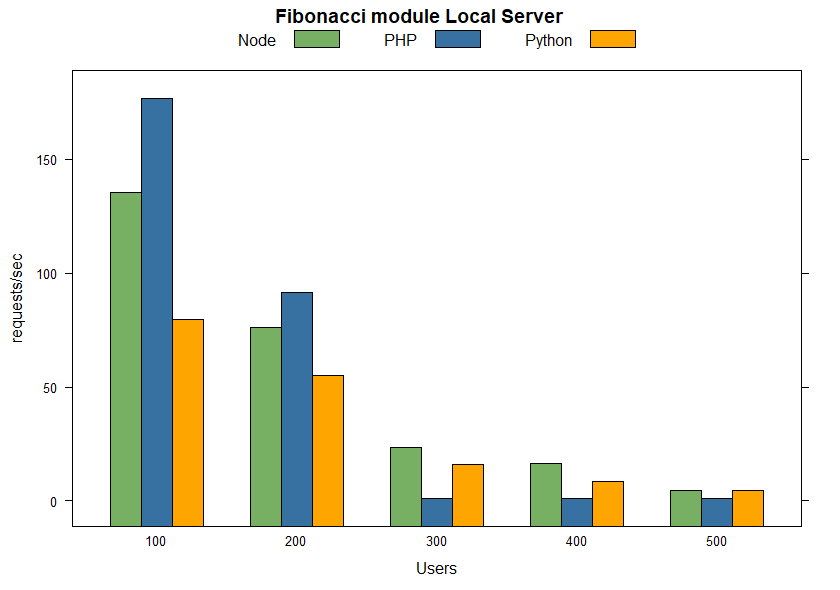
\includegraphics[width=1\textwidth]{../images/fibLocalreq.png}
		\captionsetup{justification=raggedleft, font={it, footnotesize}}
		\captionsetup{justification=justified, font={up, footnotesize}}
		\caption{Requests per second, Fibonacci module on local server}
		\label{rys1}
	\end{figure}
	\begin{figure}[H]
		\centering
		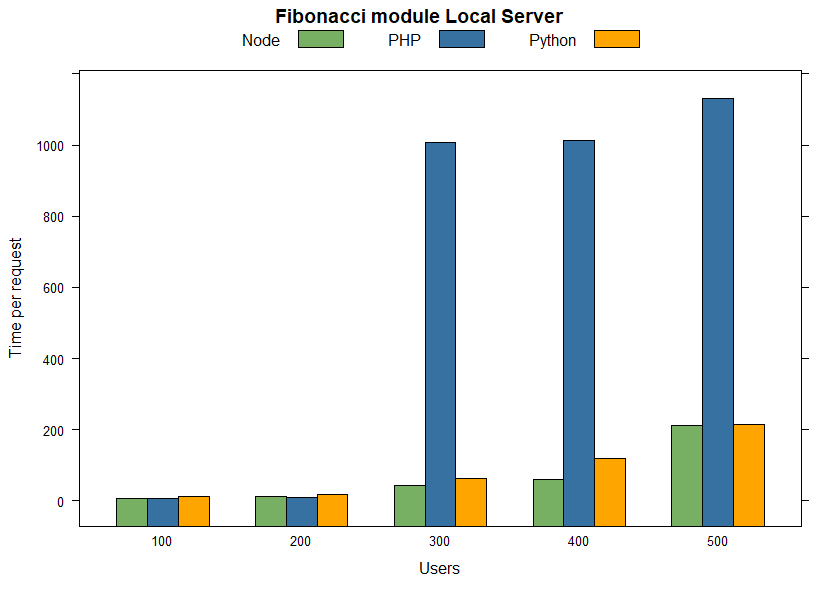
\includegraphics[width=1\textwidth]{../images/fibLocaltpr.png}
		\captionsetup{justification=raggedleft, font={it, footnotesize}}
		\captionsetup{justification=justified, font={up, footnotesize}}
		\caption{Time per request, Fibonacci module on local server}
		\label{rys1}
	\end{figure}
	\begin{figure}[H]
		\centering
		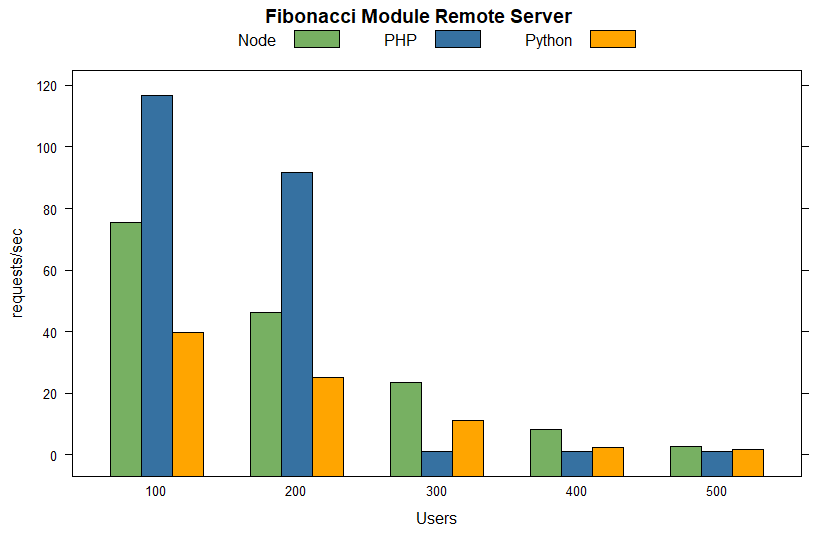
\includegraphics[width=1\textwidth]{../images/fibRemotereq.png}
		\captionsetup{justification=raggedleft, font={it, footnotesize}}
		\captionsetup{justification=justified, font={up, footnotesize}}
		\caption{Requests per second, Fibonacci module on remote server}
		\label{rys1}
	\end{figure}
	\begin{figure}[H]
		\centering
		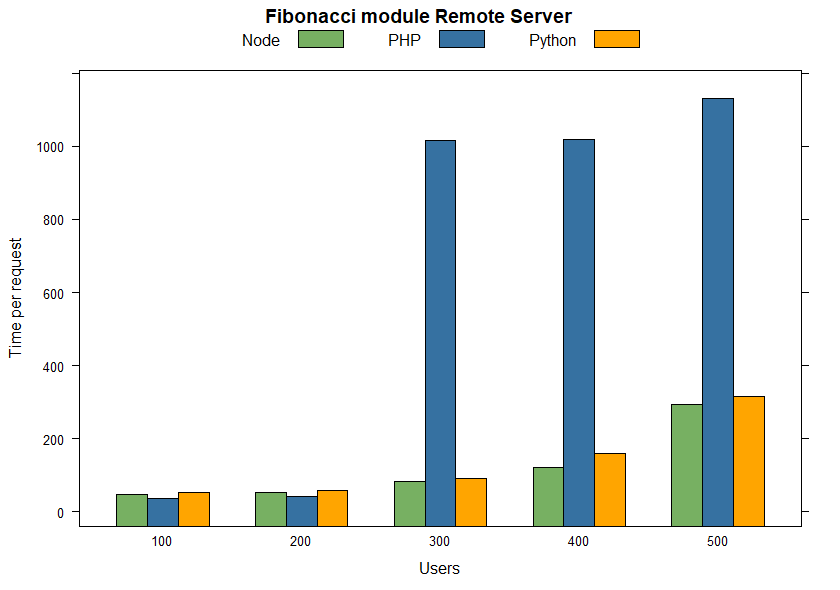
\includegraphics[width=1\textwidth]{../images/fibRemotetpr.png}
		\captionsetup{justification=raggedleft, font={it, footnotesize}}
		\captionsetup{justification=justified, font={up, footnotesize}}
		\caption{Time per request, Fibonacci module on remote server}
		\label{rys1}
	\end{figure}
	\begin{figure}[H]
		\centering
		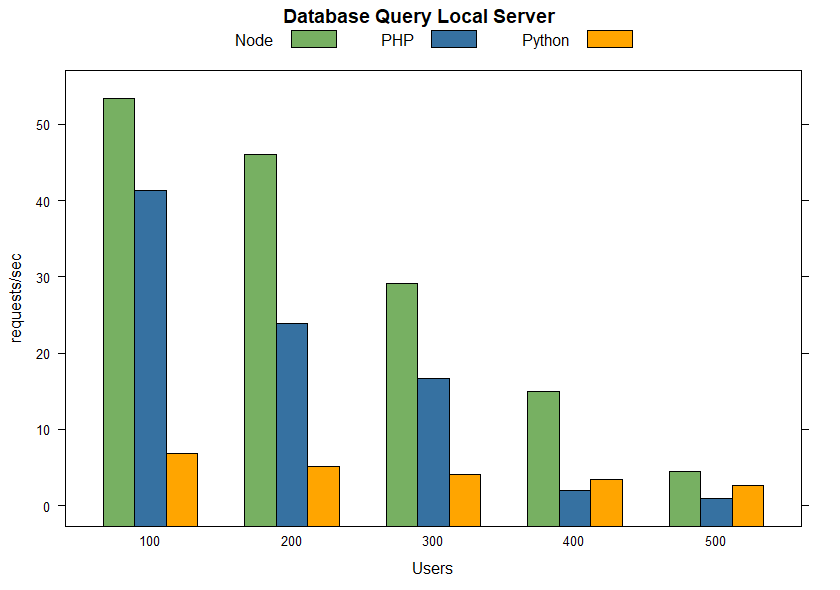
\includegraphics[width=1\textwidth]{../images/dbLocalreq.png}
		\captionsetup{justification=raggedleft, font={it, footnotesize}}
		\captionsetup{justification=justified, font={up, footnotesize}}
		\caption{Requests per second, Database query on local server}
		\label{rys1}
	\end{figure}
	\begin{figure}[H]
		\centering
		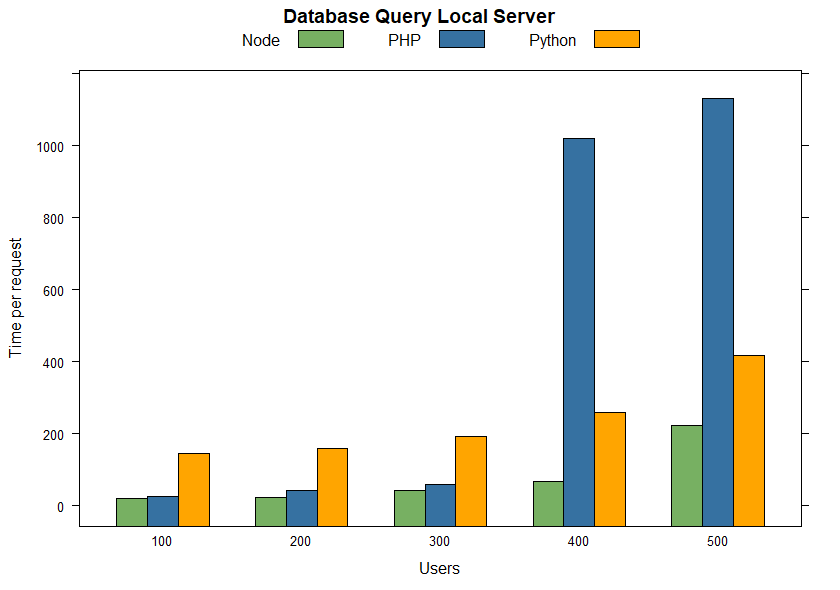
\includegraphics[width=1\textwidth]{../images/dbLocaltpr.png}
		\captionsetup{justification=raggedleft, font={it, footnotesize}}
		\captionsetup{justification=justified, font={up, footnotesize}}
		\caption{Time per request, Database query on local server}
		\label{rys1}
	\end{figure}
\end{document}